\documentclass{ximera}

%\usepackage{todonotes}

\newcommand{\todo}{}

\usepackage{tkz-euclide}
\tikzset{>=stealth} %% cool arrow head
\tikzset{shorten <>/.style={ shorten >=#1, shorten <=#1 } } %% allows shorter vectors

\usepackage{tkz-tab}  %% sign charts
\usetikzlibrary{decorations.pathreplacing} 

\usetikzlibrary{backgrounds} %% for boxes around graphs
\usetikzlibrary{shapes,positioning}  %% Clouds and stars
\usetikzlibrary{matrix} %% for matrix
\usepgfplotslibrary{polar} %% for polar plots
\usetkzobj{all}
\usepackage[makeroom]{cancel} %% for strike outs
%\usepackage{mathtools} %% for pretty underbrace % Breaks Ximera
\usepackage{multicol}

\usepackage{polynom}



\usepackage[many]{tcolorbox}  %% for titled boxes
\newtcolorbox{xbox}[1]{%
    tikznode boxed title,
    enhanced,
    arc=0mm,
    interior style={white},
    attach boxed title to top center= {yshift=-\tcboxedtitleheight/2},
    fonttitle=\bfseries,
    colbacktitle=white,coltitle=black,
    boxed title style={size=normal,colframe=white,boxrule=0pt},
    title={#1}}


\usepackage{array}
\setlength{\extrarowheight}{+.1cm}   
\newdimen\digitwidth
\settowidth\digitwidth{9}
\def\divrule#1#2{
\noalign{\moveright#1\digitwidth
\vbox{\hrule width#2\digitwidth}}}





\newcommand{\RR}{\mathbb R}
\newcommand{\R}{\mathbb R}
\newcommand{\N}{\mathbb N}
\newcommand{\Z}{\mathbb Z}

%\renewcommand{\d}{\,d\!}
\renewcommand{\d}{\mathop{}\!d}
\newcommand{\dd}[2][]{\frac{\d #1}{\d #2}}
\newcommand{\pp}[2][]{\frac{\partial #1}{\partial #2}}
\renewcommand{\l}{\ell}
\newcommand{\ddx}{\frac{d}{\d x}}
\newcommand{\ddt}{\frac{d}{\d t}}

\newcommand{\zeroOverZero}{\ensuremath{\boldsymbol{\tfrac{0}{0}}}}
\newcommand{\inftyOverInfty}{\ensuremath{\boldsymbol{\tfrac{\infty}{\infty}}}}
\newcommand{\zeroOverInfty}{\ensuremath{\boldsymbol{\tfrac{0}{\infty}}}}
\newcommand{\zeroTimesInfty}{\ensuremath{\small\boldsymbol{0\cdot \infty}}}
\newcommand{\inftyMinusInfty}{\ensuremath{\small\boldsymbol{\infty - \infty}}}
\newcommand{\oneToInfty}{\ensuremath{\boldsymbol{1^\infty}}}
\newcommand{\zeroToZero}{\ensuremath{\boldsymbol{0^0}}}
\newcommand{\inftyToZero}{\ensuremath{\boldsymbol{\infty^0}}}



\newcommand{\numOverZero}{\ensuremath{\boldsymbol{\tfrac{\#}{0}}}}
\newcommand{\dfn}{\textbf}
%\newcommand{\unit}{\,\mathrm}
\newcommand{\unit}{\mathop{}\!\mathrm}
\newcommand{\eval}[1]{\bigg[ #1 \bigg]}
\newcommand{\seq}[1]{\left( #1 \right)}
\renewcommand{\epsilon}{\varepsilon}
\renewcommand{\iff}{\Leftrightarrow}

\DeclareMathOperator{\arccot}{arccot}
\DeclareMathOperator{\arcsec}{arcsec}
\DeclareMathOperator{\arccsc}{arccsc}
\DeclareMathOperator{\si}{Si}
\DeclareMathOperator{\proj}{proj}
\DeclareMathOperator{\scal}{scal}


\newcommand{\tightoverset}[2]{% for arrow vec
  \mathop{#2}\limits^{\vbox to -.5ex{\kern-0.75ex\hbox{$#1$}\vss}}}
\newcommand{\arrowvec}[1]{\tightoverset{\scriptstyle\rightharpoonup}{#1}}
\renewcommand{\vec}{\mathbf}
\newcommand{\veci}{\vec{i}}
\newcommand{\vecj}{\vec{j}}
\newcommand{\veck}{\vec{k}}
\newcommand{\vecl}{\boldsymbol{\l}}

\newcommand{\dotp}{\bullet}
\newcommand{\cross}{\boldsymbol\times}
\newcommand{\grad}{\boldsymbol\nabla}
\newcommand{\divergence}{\grad\dotp}
\newcommand{\curl}{\grad\cross}
%\DeclareMathOperator{\divergence}{divergence}
%\DeclareMathOperator{\curl}[1]{\grad\cross #1}


\colorlet{textColor}{black} 
\colorlet{background}{white}
\colorlet{penColor}{blue!50!black} % Color of a curve in a plot
\colorlet{penColor2}{red!50!black}% Color of a curve in a plot
\colorlet{penColor3}{red!50!blue} % Color of a curve in a plot
\colorlet{penColor4}{green!50!black} % Color of a curve in a plot
\colorlet{penColor5}{orange!80!black} % Color of a curve in a plot
\colorlet{fill1}{penColor!20} % Color of fill in a plot
\colorlet{fill2}{penColor2!20} % Color of fill in a plot
\colorlet{fillp}{fill1} % Color of positive area
\colorlet{filln}{penColor2!20} % Color of negative area
\colorlet{fill3}{penColor3!20} % Fill
\colorlet{fill4}{penColor4!20} % Fill
\colorlet{fill5}{penColor5!20} % Fill
\colorlet{gridColor}{gray!50} % Color of grid in a plot

\newcommand{\surfaceColor}{violet}
\newcommand{\surfaceColorTwo}{redyellow}
\newcommand{\sliceColor}{greenyellow}




\pgfmathdeclarefunction{gauss}{2}{% gives gaussian
  \pgfmathparse{1/(#2*sqrt(2*pi))*exp(-((x-#1)^2)/(2*#2^2))}%
}


%%%%%%%%%%%%%
%% Vectors
%%%%%%%%%%%%%

%% Simple horiz vectors
\renewcommand{\vector}[1]{\left\langle #1\right\rangle}


%% %% Complex Horiz Vectors with angle brackets
%% \makeatletter
%% \renewcommand{\vector}[2][ , ]{\left\langle%
%%   \def\nextitem{\def\nextitem{#1}}%
%%   \@for \el:=#2\do{\nextitem\el}\right\rangle%
%% }
%% \makeatother

%% %% Vertical Vectors
%% \def\vector#1{\begin{bmatrix}\vecListA#1,,\end{bmatrix}}
%% \def\vecListA#1,{\if,#1,\else #1\cr \expandafter \vecListA \fi}

%%%%%%%%%%%%%
%% End of vectors
%%%%%%%%%%%%%

%\newcommand{\fullwidth}{}
%\newcommand{\normalwidth}{}



%% makes a snazzy t-chart for evaluating functions
%\newenvironment{tchart}{\rowcolors{2}{}{background!90!textColor}\array}{\endarray}

%%This is to help with formatting on future title pages.
\newenvironment{sectionOutcomes}{}{} 



%% Flowchart stuff
%\tikzstyle{startstop} = [rectangle, rounded corners, minimum width=3cm, minimum height=1cm,text centered, draw=black]
%\tikzstyle{question} = [rectangle, minimum width=3cm, minimum height=1cm, text centered, draw=black]
%\tikzstyle{decision} = [trapezium, trapezium left angle=70, trapezium right angle=110, minimum width=3cm, minimum height=1cm, text centered, draw=black]
%\tikzstyle{question} = [rectangle, rounded corners, minimum width=3cm, minimum height=1cm,text centered, draw=black]
%\tikzstyle{process} = [rectangle, minimum width=3cm, minimum height=1cm, text centered, draw=black]
%\tikzstyle{decision} = [trapezium, trapezium left angle=70, trapezium right angle=110, minimum width=3cm, minimum height=1cm, text centered, draw=black]


\title[Dig-In:]{Basic antiderivatives}

\begin{document}
\begin{abstract}
  We introduce antiderivatives.
\end{abstract}
\maketitle


Computing derivatives is not too difficult. At this point, you should
be able to take the derivative of almost any function you can write
down. However, undoing derivatives is much harder. This process of
undoing a derivative is called taking an \textit{antiderivative}.

\begin{definition}
A function $F$ is called an \dfn{antiderivative} of $f$ on an
interval if
\[
F'(x) = f(x)
\]
for all $x$ in the interval.
\end{definition}

%% \begin{question} BADBAD
%%   Give three antiderivatives of $f(x) = 2x$.  
%%   \[F_1(x) = \answer[antiderivative]{2x} \]
%%   \[F_2(x) = \answer[antiderivative]{2x} \]
%%   \[F_3(x) = \answer[antiderivative]{2x} \]
%% \end{question}

\begin{question}
  How many antiderivatives does $f(x) = 2x$ have?
  \begin{prompt}
  \begin{multipleChoice}
    \choice{none}
    \choice{one}
    \choice[correct]{infinitely many}
  \end{multipleChoice}
  \end{prompt}
  \begin{feedback}
   \begin{image}
          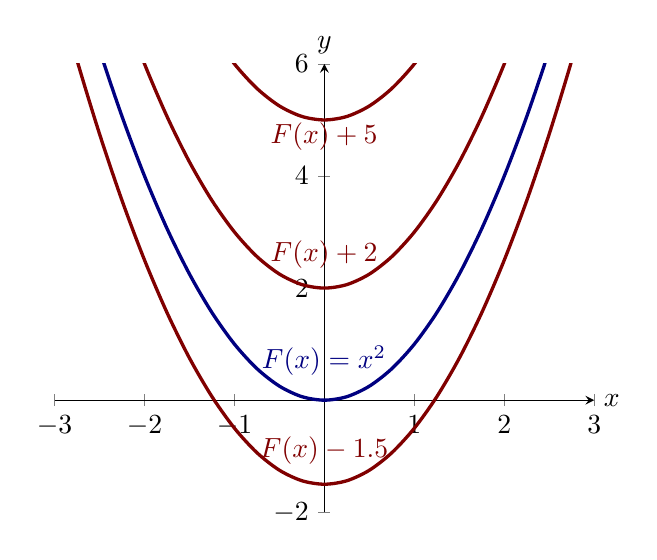
\begin{tikzpicture}
	    \begin{axis}[
            domain=-3:3,
            xmin=-3, xmax=3,
            ymin=-2, ymax=6
         ,
            axis lines =middle, xlabel=$x$, ylabel=$y$,
            every axis y label/.style={at=(current axis.above origin),anchor=south},
            every axis x label/.style={at=(current axis.right of origin),anchor=west},
          ]
	  \addplot [very thick, penColor, smooth] {x^2};
         \addplot [very thick, penColor2, smooth] {x^2-1.5};
    \addplot [very thick, penColor2, smooth] {x^2+2};
        \addplot [very thick, penColor2, smooth] {x^2+5};
          \node at (axis cs:-0.004,2.6) [penColor2] {$F(x)+2$};
          \node at (axis cs:-0.004,.7) [penColor] {$F(x)=x^2$};
          \node at (axis cs:-0.004,-0.9) [penColor2] {$F(x)-1.5$};
            \node at (axis cs:-0.004,4.7) [penColor2] {$F(x)+5$};
        \end{axis}
\end{tikzpicture}
%% \caption{A plot of $f(x)=x^2$ and $f^{-1}(x) = \sqrt{x}$. While
%%   $f(x)=x^2$ is not one-to-one on $\RR$, it is one-to-one on
%%   $[0,\infty)$.}
%% \label{plot:fxn and inverse x^2}
\end{image}
    The functions $x^2$, $x^2-1.5$, $x^2+2$, $x^2+5$ and so on, are all
    antiderivatives of $2x$.
    
     It is clear that any function $x^2+C$, where $C$ is a constant, is an antiderivative of $f$. Why?
    Because, $(x^2+C)'=2x=f(x)$.
    
     Could there exist any other antiderivative of $f$, call it $G$, such that $G(x)$ is not a sum of $x^2$ and a constant?
    In that case, for all $x$  we would have
  \[
  (G(x)-x^2)' = G'(x)-2x=f(x)-2x= \answer[given]{0}\\
\]
  \end{feedback}
  Recall: Any function whose derivative is equal to $0$ on some interval is equal to a constant on that interval.
  This means that the function $G(x)-x^2=C$, for some constant $C$. This implies that $G(x)=x^2+C$, for all x.
\end{question}


\begin{theorem}[The Family of Antiderivatives]\label{theorem:FOA}

If $F$ is an antiderivative of $f$, then the function $f$ has a whole \textbf{family of antiderivatives}. Each antiderivative of $f$ is the sum of $F$ and some constant $C$.
\end{theorem}

So, when we write $F(x)+C$, we denote the entire family of
antiderivatives of $f$.  Alternative notation for this family of
antiderivatives was introduced by \link[G.W.\ Leibniz]{https://en.wikipedia.org/wiki/Gottfried_Wilhelm_Leibniz} (1646-1716):
 
\begin{definition}\index{antiderivative!notation}\index{indefinite integral}
Let $f$ be a function. The family of of \emph{all} antiderivatives of $f$ is denoted by
\[
\int f(x) \d x. 
\]

This is called the
\dfn{indefinite integral} of $f$.
\end{definition}
It follows that
\[
\int f(x) \d x =F(x)+C,
\]
where $F$ is any antiderivative of $f$ and $C$ is an arbitrary constant.

Now we are ready to "integrate" some famous functions.


Fill out these basic antiderivatives. Note each of these examples comes
directly from our knowledge of basic derivatives.

%% BADBAD - we want this back.
%% \begin{theorem}[Basic Antiderivatives]\label{theorem:basicAnti} \hfil
%% %\begin{multicols}{3}
%% %\todo{Originally this was done with the multicols environment}
%% \begin{question}
%% \begin{itemize}
%% \item An antiderivative of  $k$ is $\answer[antiderivative]{k}$
%% \item An antiderivative of $x^n$, for $n \neq -1$,  is $\answer[antiderivative]{x^n}$
%% \item An antiderivative of  $e^x$ is $\answer[antiderivative]{e^x}$
%% % Is this really needed? \item $\int a^x \d x= \frac{a^x}{\ln(a)}+C$.
%% \item An antiderivative of  $\frac{1}{x}$ is $\answer[antiderivative]{1/x}$. (Be careful that your answer makes works on the full domain, not just $(0,\infty)$)
%% \item An antiderivative of $\cos(x)$ is  $\answer[antiderivative]{\cos(x)}$.
%% \item An antiderivative of $\sin(x)$ is $\answer[antiderivative]{\sin(x)}$.  
%% \item An antiderivative of $\tan(x)$ is $\answer[antiderivative]{\tan(x)}$.  
%% \item An antiderivative of $\sec^2(x)$ is $\answer[antiderivative]{\sec^2(x)}$. 
%% \item An antiderivative of $\csc^2(x)$ is $\answer[antiderivative]{\csc^2(x)}$.
%% \item An antiderivative of $\sec(x)\tan(x)$ is $\answer[antiderivative]{\sec(x)\tan(x)}$.
%% \item An antiderivative of $\csc(x)\cot(x)$ is $\answer[antiderivative]{\csc(x)\cot(x)}$.
%% \item An antiderivative of $\frac{1}{x^2+1}$ is $\answer[antiderivative]{\frac{1}{1+x^2}}$.
%% \item An antiderivative of $\frac{1}{\sqrt{1-x^2}}$ is $\answer[antiderivative]{\frac{1}{\sqrt{1-x^2}}}$.
%% \end{itemize}
%% \end{question}
%% \end{theorem}

\begin{theorem}[Basic Indefinite Integrals]\index{antiderivatives}\index{indefinite integral}\hfil
\begin{itemize}
\item $\int k \d x= \answer[given]{k x}+C$
\item $\int \frac{1}{x} \d x= \answer[given]{\ln|x|}+C$
\item $\int x^n \d x= \answer[given]{\frac{x^{n+1}}{n+1}}+C\qquad(n\ne-1)$
\item $\int e^x \d x= \answer[given]{e^x} + C$
\item $\int a^x \d x= \answer[given]{\frac{a^x}{\ln(a)}}+C$
\item $\int \cos(x) \d x = \answer[given]{\sin(x)} + C$
\item $\int \sin(x) \d x = \answer[given]{-\cos(x)} + C$  
\item $\int \sec^2(x) \d x = \answer[given]{\tan(x)} + C$
\item $\int \csc^2(x) \d x = \answer[given]{-\cot(x)} + C$
\item $\int \sec(x)\tan(x) \d x = \answer[given]{\sec(x)} + C$
\item $\int \csc(x)\cot(x) \d x = \answer[given]{-\csc(x)} + C$
\item $\int \frac{1}{x^2+1}\d x = \answer[given]{\arctan{x}} + C$
\item $\int \frac{1}{\sqrt{1-x^2}}\d x= \answer[given]{\arcsin{x}}+C$
\end{itemize}
\end{theorem}


It may seem that one could simply memorize these antiderivatives and
antidifferentiating would be as easy as differentiating. This is
\textbf{not} the case. The issue comes up when trying to combine these
functions.  When taking derivatives we have the \textit{product rule}
and the \textit{chain rule}. The analogues of these two rules are much
more difficult to deal with when taking antiderivatives. However, not
all is lost.

Consider the following example.
\begin{example}
  Find  an antiderivative of the function $h$ defined by expression
  
   $h(x)=\cos{x}+\frac{1}{x}$, for all $x$ in some interval $I$.
  \begin{multipleChoice}
    \choice{$H(x)=\cos{x}+\frac{1}{x}$}
    \choice{$H(x)=\sin{x}+\frac{1}{x^2}$}
    \choice[correct]{$H(x)=\sin{x}+\ln{x}$}
  \end{multipleChoice}
  \begin{feedback}
    Differentiate each choice.
    
     In the last choice we get $H'(x)=\cos{x}+\frac{1}{x}=h(x)$.
  \end{feedback}
\end{example}
It is easy to recognize an antiderivative: we just have to differentiate it, and check wether $H'(x)=h(x)$, for all $x$ in $I$.

Notice, that the function $h$ is the sum of the two functions, $f$ and $g$, where $f(x)=\cos{x}$ and $g(x)=\frac{1}{x}$, for $x$ in $I$.

We know antiderivatives of both functions:  $F(x)=\sin{x}$ and $G(x)=\ln{x}$,  for $x$ in $I$, are antiderivatives of $f$ and $g$, respectively.
So, in this example we see that the function  $F+G$ is an antiderivative of $f+g$.
In other words, "the sum of antiderivatives is an antiderivative of a sum".

Is this true in general? 

Let's check whether this rule holds for any eligible pair of functions $f$ and $g$ defined on some interval $I$.
 \begin{question}
Let $f$, $g$, $F$ and $G$ be four functions defined on some interval $I$ such that $F$ is an antiderivative of $f$ and $G$ is an antiderivative of $g$, i.e.

$F'(x)=f(x)$ and $G'(x)=g(x)$ for all $x$ in some interval $I$.

  Find an antiderivative of the function $f+g$.
    \begin{hint}
    Differentiate the function $F+G$.
     \end{hint}
     Since
     $\left(F(x)+G(x)\right)'=F'(x)+G'(x)=f(x)+g(x)$,
     it follows that  $F+G$ is an antiderivative of $f+g$. 
     
 To summarize: The sum of antiderivatives is an antiderivative of a sum. 
\end{question}
We have proved the following theorem.

\begin{theorem}[The Sum Rule for Antiderivatives]\label{theorem:SRA}
If $F$ is an antiderivative of $f$ and $G$ is an antiderivative of
$g$, then $F+G$ is an antiderivative of $f+g$.

We can write equivalently, using indefinite integrals, 

$\int \left(f(x)+g(x)\right) \d x= \int f(x)\d x +\int g(x) \d x$.
\end{theorem}

Next, we will try to prove an analogue of the constant multiple rule for derivatives.
Let's consider the following example.
\begin{example}
  Find  an antiderivative of the function $h$, where
   $h(x)=5\sec^{2}{x}$,  for all $x$ in some interval $I$.
  \begin{multipleChoice}
  \choice[correct]{$H(x)=5\tan{x}$}
    \choice{$H(x)=5\sec^{2}{x}$}
    \choice{$H(x)=\sec^{2}{5x}$}
  \end{multipleChoice}
  \begin{feedback}
    Differentiate each choice for $H(x)$.  In the first choice we get
    $H'(x)=5\sec^{2}{x}=h(x)$.
  \end{feedback}
\end{example}
It is easy to recognize an antiderivative: we just have to differentiate it, and check wether $H'(x)=h(x)$, for all $x$ in $I$.

Notice, in this example the function $h$ is a constant multiple of $f$, 

where $f(x)=\sec^{2}{x}$. On the other hand, we know that the function $F$, defined by 
$F(x)=\tan{x}$ is an antiderivative of $f$.

If we  differentiate the function $5F$, we get that

  $\left(5F(x)\right)'=\left(5\tan{x}\right)'=5\left(\tan{x}\right)'=5\sec^{2}{x}=5f(x)$, for $x$ in $I$.
  
  In other words, ``a constant multiple of an antiderivative is an antiderivative of a constant multiple of a function.''
Is this always true?

Let's check whether this rule holds for  any constant $k$ and any eligible  function $f$ defined on some interval $I$.
 \begin{question}
Let $k$ be a constant, let $f$ be a function defined on some interval $I$ and let $F$ be an antiderivative of $f$, i.e.

$F'(x)=f(x)$, for all  $x$ in some interval $I$.

  Find an antiderivative of the function $k f$.
    \begin{hint}
    Differentiate the function $kF$.
     \end{hint}
     Since $\left(kF(x)\right)'=kF'(x)=kf(x)$, it follows that $kF$ is
     an antiderivative of $kf$.
 To summarize: The constant multiple of an antiderivative is an antiderivative of a constant multiple of a function. 
\end{question}
We have proved the following theorem.
\begin{theorem}[The Constant Multiple Rule for Antiderivatives]\label{theorem:CMRA}
If $F$ is an antiderivative of $f$, and $k$ is a constant, then $kF$
is an antiderivative of $kf$.

We can write equivalently, using indefinite integrals, 
$\int kf(x) \d x= k\int f(x)\d x$.
\end{theorem}
Let's put these rules and our knowledge of basic derivatives to work.
\begin{example}
Find the antiderivative of $3 x^7$.
\begin{explanation}
By the theorems above , we see that
\begin{align*}
\int 3 x^7 \d x &= 3 \int x^7 \d x\\
&= 3 \cdot \answer[given]{\frac{x^8}{8}}+C.
\end{align*}
\end{explanation}
\end{example}
The sum rule for antiderivatives allows us to integrate
term-by-term. Let's see an example of this.

\begin{example}
Compute:
\[
\int \left(x^4 + 5x^2 - \cos(x)\right) \d x
\]
\begin{explanation}
Let's start by simplifying the problem using the sum rule 
 and constant multiple rule for antiderivatives, 
\begin{align*}
\int &\left(x^4 + 5x^2 - \cos(x)\right) \d x\\
&= \int x^4 \d x + 5\int x^2 \d x - \int \cos(x) \d x.
\end{align*}
Now we may integrate term-by-term to find
\[
= \answer[given]{\frac{x^5}{5} + \frac{5x^3}{3}  - \sin(x)}+C.
\]
\end{explanation}
\end{example}


\begin{warning}
While the sum rule for antiderivatives allows us to integrate
term-by-term, we cannot integrate \textit{factor-by-factor}, meaning
that in general
\[
\int f(x)g(x) \d x \ne \int f(x) \d x\cdot \int g(x) \d x.
\]
\end{warning}


\begin{example}
  A student claims that $\int 2x \cos(x) \d x = x^2 \sin(x) +C$.  Determine whether the student is correct or incorrect.
  
  \begin{explanation}
    If the student were correct, then the derivative of $x^2 \sin(x) +C$ with respect to $x$ would have to be $2x \cos(x)$.  However:
    
      \[\ddx x^2 \sin(x) = \answer[given]{2x \sin(x) +x^2 \cos(x)} \]
      
 Hence, the student is incorrect!
  \end{explanation}
\end{example}






\section{Computing antiderivatives}


Unfortunately, we cannot tell you how to compute every antiderivative,
we view them as a sort of \textit{puzzle}. Later we will learn a
hand-full of techniques for computing antiderivatives. However, a
robust and simple way to compute antiderivatives is guess-and-check.


%\begin{guessingAntiderivatives}\hfil
\paragraph{Tips for guessing antiderivatives}
\begin{enumerate}
\item If possible, express the function that you are integrating in a form that is convenient for integration.
\item Make a guess for the antiderivative.
\item Take the derivative of your guess.
\item Note how the above derivative is different from the function
  whose antiderivative you want to find.
\item Change your original guess by \textbf{multiplying} by constants
  or by \textbf{adding} in new functions.
\end{enumerate}
%\end{guessingAntiderivatives}


\begin{example}
Compute:
\[
\int \frac{\sqrt{x}+1+x}{x} \d x
\]
\begin{explanation}
Before guessing the solution, let's express  the function in the form convenient for integration. Due to Sum Rule, it is more convenient to have a sum of functions, instead of a single, complicated term.
\begin{align*}
  \int \frac{\sqrt{x}+1+x}{x} \d x &=\int \left(\frac{\sqrt{x}}{x}+\frac{1}{x}+\frac{x}{x}\right) \d x\\
  &=\int \left(\frac{1}{\sqrt{x}}+\frac{1}{x}+1\right) \d x\\
  &=\int \left(x^{-\frac{1}{2}}+\frac{1}{x}+1\right) \d x
\end{align*}
Now, we can apply the Sum Rule.
\[
\int \left(x^{-\frac{1}{2}}+\frac{1}{x}+1\right) \d x=\int x^{-\frac{1}{2}}\d x+\int\frac{1}{x}\d x+\int1 \d x
\]
Now we can finish the problem.
\[
\int \frac{\sqrt{x}+1+x}{x} \d x= \answer[given]{2}\sqrt{x}+\ln{x}+ \answer[given]{x} + C.
\]
\end{explanation}
\end{example}
\begin{example}
  Compute:
  \[
  \int \cos{(4x)} \d x
  \]
  \begin{explanation}
    Start with a guess of 
    \[
    \int \cos{(4x)} \d x \approx \sin{(4x)}.
    \]
    Take the derivative of your guess to see if it is correct:
    \[
    \ddx  \sin{(4x)} = 4 \cos{(4x)}.
    \]
    We're off by a factor of $\frac{1}{4}$, so multiply your guess by this constant
    to get the solution,
    \[
  \int \cos{(4x)} \d x = \answer[given]{\frac{1}{4}\sin{(4x)}}+C.
    \]
\end{explanation}
\end{example}
\begin{example}
  Compute:
  \[
  \int 3x^2\sin{(x^3 -6)} \d x
  \]
  \begin{explanation}
    Start with a guess of 
    \[
 \int 3x^2\sin{(x^3 -6)} \d x \approx -\cos{(x^3 -6)}.
    \]
    Take the derivative of your guess to see if it is correct:
    \[
    \ddx \left(-\cos{(x^3 -6)}\right) = 3x^2\sin{(x^3 -6)}.
    \]
   Therefore,
    \[
    \int 3x^2\sin{(x^3 -6)} \d x
 =- \cos{(\answer[given]{x^3 -6})}+C.
    \]
\end{explanation}
\end{example}

\begin{example}
  Compute:
  \[
  \int x^2\sin{(x^3 -6)} \d x
  \]
  \begin{explanation}
    Start with a guess of 
    \[
 \int x^2\sin{(x^3 -6)} \d x \approx -\cos{(x^3 -6)}.
    \]
    Take the derivative of your guess to see if it is correct:
    \[
    \ddx \left(-\cos{(x^3 -6)}\right) = 3x^2\sin{(x^3 -6)}.
    \]
    We're off by a factor of $1/3$, so multiply our guess by this constant
    to get the solution,
    \[
    \int x^2\sin{(x^3 -6)} \d x
 =- \answer[given]{\frac{1}{3}}\cos{(x^3 -6)}+C.
    \]
\end{explanation}
\end{example}

\begin{example}
  Compute:
  \[
  \int \frac{x^3}{\sqrt{x^4 -6}} \d x
  \]
  \begin{explanation}
    Start by rewriting the indefinite integral as
    \[
    \int x^3\left(x^4 -6\right)^{-1/2} \d x.
    \]
    Now start with a guess of 
    \[
    \int x^3\left(x^4 -6\right)^{-1/2} \d x \approx \left(x^4 -6\right)^{1/2}.
    \]
    Take the derivative of your guess to see if it is correct:
    \[
    \ddx  \left(x^4 -6\right)^{1/2} = (4/2)x^3\left(x^4 -6\right)^{-1/2}.
    \]
    We're off by a factor of $2/4$, so multiply our guess by this constant
    to get the solution,
    \[
    \int \frac{x^3}{\sqrt{x^4 -6}} \d x = \answer[given]{\frac{1}{2}}(x^4 -6)^{1/2}+C.
    \]
\end{explanation}
\end{example}

\begin{example}
Compute:
\[
\int xe^{x^2} \d x
\]
\begin{explanation}
We try to guess the antiderivative. Start with a guess of
\[
\int xe^{x^2} \d x \approx e^{x^2}.
\]
Take the derivative of your guess to see if it is correct:
\[
\ddx e^{x^2} = 2xe^{x^2} .
\]
Ah! So we need only multiply our original guess by $\frac{1}{2}$.  We now
find
\[
\int xe^{x^2} \d x =\answer[given]{\frac{1}{2}}e^{x^2} + C.
\]
\end{explanation}
\end{example}
\begin{example}
Compute:
\[
\int \frac{21x^2}{7x^3 + 3} \d x
\]
\begin{explanation}
We notice that the numerator is the derivative of the denominator, i.e., the function that we are integrating has the form $\frac{f'(x)}{f(x)}$.
\[
\int \frac{21x^2}{7x^3 + 3} \d x = \ln(7x^3+3).
\]
Take the derivative of your guess to see if it is correct:
\[
\ddx \ln(7x^3+3) = \frac{21x^2}{7x^3 + 3}.
\]
Therefore,
\[
\int \frac{21x^2}{7x^3 + 3} \d x = \ln{(\answer[given]{7x^3+3})}+C.
\]
\end{explanation}
\end{example}
\begin{example}
Compute:
\[
\int \frac{2x^2}{7x^3 + 3} \d x
\]
\begin{explanation}
We'll start with a guess of
\[
\int \frac{2x^2}{7x^3 + 3} \d x \approx \ln(7x^3+3).
\]
Take the derivative of your guess to see if it is correct:
\[
\ddx \ln(7x^3+3) = \frac{21x^2}{7x^3 + 3}.
\]
We are only off by a factor of $2/21$, so we need to multiply our
original guess by this constant to get the solution,
\[
\int \frac{2x^2}{7x^3 + 3} \d x = \answer[given]{(2/21)\ln(7x^3+3)}+C.
\]
\end{explanation}
\end{example}

\section{Final thoughts}
Computing antiderivatives is a place where insight and rote
computation meet. We cannot teach you a method that will always
work. Moreover, merely \emph{understanding} the examples above will
probably not be enough for you to become proficient in computing
antiderivatives. You must practice, practice, practice!

\section{Differential equations}

Differential equations show you relationships between rates of
functions.



A \textit{differential equation}\index{differential equation} is
simply an equation with a derivative in it. Here is an example:
\[
a\cdot f'(x)+ b\cdot f(x) = g(x). 
\]
\begin{question}
	Which one is a differential equation?
	\begin{multipleChoice}
		\choice{$x^2+3x-1=0$}
		\choice[correct]{$f'(x)=x^2+3x-1$}
		\choice{$f(x)=x^2+3x-1$}  
	\end{multipleChoice}
\end{question}

When a mathematician solves a differential equation, they are finding
\textit{functions} satisfying the equation.
\begin{question}
	Which of the following functions solve the differential equation
	\[
	f'(x) = f(x)?
	\]
	\begin{selectAll}
		\choice{$f(x) = \sin(x)$}
		\choice{$f(x) = x^2$}
		\choice[correct]{$f(x) = e^x$}
		\choice[correct]{$f(x) =6 e^x$}
		\choice{$f(x) = e^{-x}$}
		\choice{$f(x) = \tan(x)$}
	\end{selectAll}
\end{question}
\begin{remark}
	We can directly check that any function $f(x)=Ce^x$ is a solution to our differential equation $f'(x)=f(x)$. Could there be any others? It turns out that these are the \textit{only} solutions. But showing that we didn't miss any is a bit tricky.
	\begin{expandable}
		\begin{explanation}
			Well, suppose we have some mysterious function $f$ and all we know is that $f'(x)=f(x)$. Let's define a new function $g(x)=f(x)/e^x$. Since our denominator is never 0, the quotient rule tells us that
			\[
			g'(x)= \frac{e^x f'(x)- f(x) e^x}{(e^x)^2} = \frac{e^x\left(f'(x)- f(x)\right)}{(e^x)^2} = \frac{e^x\cdot 0}{(e^x)^2}=0.
			\]
			But we know that a function with a 0 derivative is constant, so $g(x)=C$. Plugging this back into our formula for $g(x)$ tells us that $C=f(x)/e^x$. Now we rearrange to get $f(x)=Ce^x$.
			
			This shows us that any solution to our differential equation \textit{must} be one of the functions we've already found. Our argument relies on some features that are special to this problem; proving that we've found all the possible solutions to an arbitrary differential equation is a very difficult task!   
		\end{explanation} 
	\end{expandable}
\end{remark}

A function $Ce^x$ is called a \dfn{general solution} of the differential equation. Since there are infinitely many solutions to a differential equation, we can impose an additional condition (say $f(0)=1$), called an \dfn{initial condition}. When we are asked to find a function $f$ that satisfies both the differential equation (DE) and the initial condition (IC), this is called an \dfn{initial value problem} (IVP). Let's try one out.
\begin{example}
	Solve the initial value problem (IVP):
	\begin{align*}
		f'(x) & = f(x) && \text{(DE)}  \\
		f(0) & = 1 && \text{(IC)} 
	\end{align*}
	\begin{explanation}
		The figure below shows several solutions of the differential equation. 
		\begin{image}
			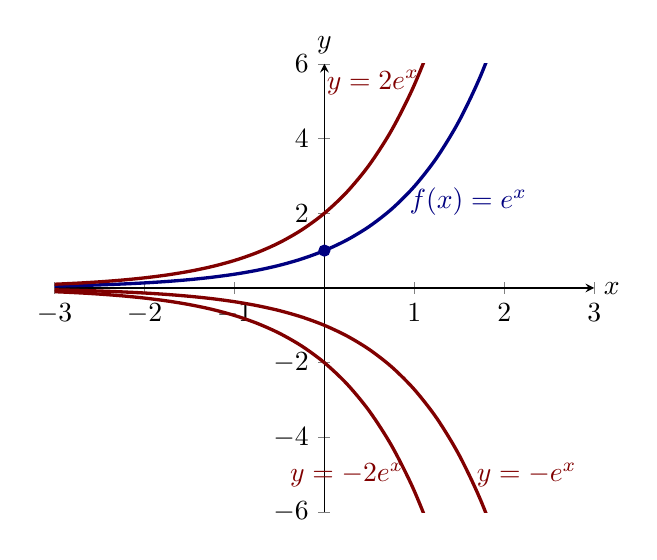
\begin{tikzpicture}
			\begin{axis}[
			domain=-3:3,
			xmin=-3, xmax=3,
			ymin=-6
			, ymax=6,
			axis lines =middle, xlabel=$x$, ylabel=$y$,
			every axis y label/.style={at=(current axis.above origin),anchor=south},
			every axis x label/.style={at=(current axis.right of origin),anchor=west},
			]
			\addplot [very thick, penColor, smooth] {e^x};
			\addplot [very thick, penColor2, smooth] {2*e^x};
			\addplot [very thick, penColor2, smooth] {-2*e^x};
			\addplot [very thick, penColor2, smooth] {-e^x};
			\addplot [color=penColor,fill=penColor,only marks,mark=*] coordinates{(0,1)};  %% closed hole 
			\node at (axis cs:1.6,2.3) [penColor] {$f(x)=e^x$};
			\node at (axis cs:2.25,-5) [penColor2] {$y=-e^x$};
			\node at (axis cs:0.25,-5) [penColor2] {$y=-2e^x$};
			\node at (axis cs:0.54,5.5) [penColor2] {$y=2e^x$};
			\end{axis}
			\end{tikzpicture}
		\end{image}
		The figure suggests that the only solution to the initial value problem is the function $f(x)=e^x$.
		We can verify this result.
		
		Since all solutions of the differential equation have the form $f(x)=Ce^x$ and $f(0)=1$, it follows that 
		\[
		Ce^0 = 1.
		\]
		Therefore,
		\[
		C = \answer[given]{1}.
		\]
		So, the \textbf{unique} solution to the given initial value problem is the function $f(x)=e^x$.
	\end{explanation}
\end{example}

\begin{example}
	Solve the initial value problem (IVP):
	\begin{align*}
		f'(x) & = \sin{x}  \\
		f(0) & = -1 
	\end{align*}
	\begin{explanation}
		First, we have to solve the differential equation. The solution is clearly an antiderivative of $\sin{x}$.
		\[
		f(x)=-\answer[given]{\cos{x}}+C,
		\]
		where $C$ is an arbitrary constant. We have found the general solution of the DE  and this family of solutions is illustrated by the figure below. 
		\begin{image}
			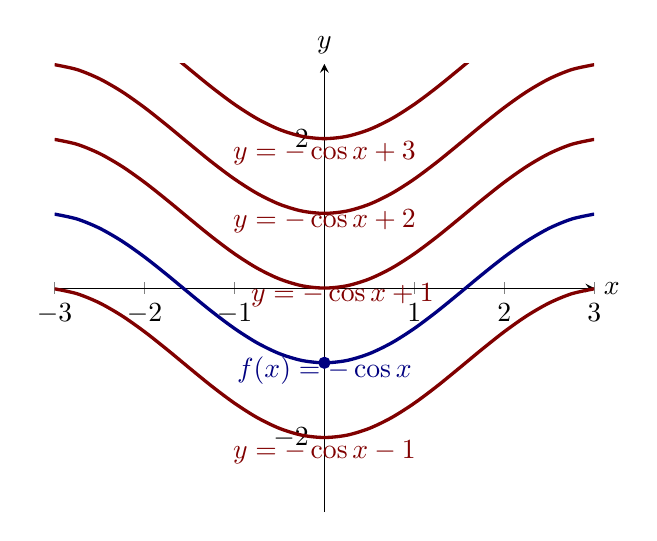
\begin{tikzpicture}
			\begin{axis}[
			domain=-3:3,
			xmin=-3, xmax=3,
			ymin=-3, ymax=3,
			axis lines =middle, xlabel=$x$, ylabel=$y$,
			every axis y label/.style={at=(current axis.above origin),anchor=south},
			every axis x label/.style={at=(current axis.right of origin),anchor=west},]
			\addplot [very thick, penColor, smooth] {-cos(deg(x))};
			\addplot [very thick, penColor2, smooth] {1-cos(deg(x))};
			\addplot [very thick, penColor2, smooth] {3-cos(deg(x))};
			\addplot [very thick, penColor2, smooth] {2-cos(deg(x))};
			\addplot [very thick, penColor2, smooth] {-1-cos(deg(x))};
			\addplot [color=penColor,fill=penColor,only marks,mark=*] coordinates{(0,-1)};  %% closed hole 
			\node at (axis cs:0,-1.1) [penColor] {$f(x)=-\cos{x}$};
			\node at (axis cs:0,-2.2) [penColor2] {$y=-\cos{x}-1$};
			\node at (axis cs:0.2,-0.1) [penColor2] {$y=-\cos{x}+1$};
			\node at (axis cs:0,0.9) [penColor2] {$y=-\cos{x}+2$};
			\node at (axis cs:0,1.8) [penColor2] {$y=-\cos{x}+3$};
			\node at (axis cs:0.54,5.5) [penColor2] {$y=2e^x$};
			\end{axis}
			\end{tikzpicture}
		\end{image}
		Now we must find the solution that also satisfies the initial condition 
		$f(0)=-1$.
		
		Since
		\[
		f(0)=\answer[given]{-1}+C,
		\]
		it follows that
		\[
		-1=\answer[given]{-1}+C.
		\]
		Therefore,
		\[
		C=\answer[given]{0}.
		\]
		The function 
		\[
		f(x)=\answer[given]{-\cos{x}}.
		\]
		is the solution of the initial value problem and it is shown in the figure above.
	\end{explanation}
\end{example}
\end{document}
